\begin{frame}{Loading}
    \begin{tabular}{m{0.65\textwidth} m{0.3\textwidth}}
        \underline{Circuit with loading: voltage divider} & \multirow{2}{*}{
            \begin{circuitikz}[scale=0.6, transform shape]
                \draw (0,0) node[label={left:$V_{in}$}] {} to[short] (1, 0)
                (1, 0) to[R=$R_1$] (1, -2)
                (1, -2) to[short] (2, -2) node[label={right:$V_{out}$}] {}
                (1, -2) to[R=$R_2$] (1, -4) node[ground] {};
            \end{circuitikz}
        } \\[5pt]
        With voltage dividers: $V_{out}$ depends on the \textbf{load}, or the \textit{current drawn from the $V_{out}$ terminal}. & \\[50pt]
        \underline{Circuit w/o loading: op-amp} & \multirow{2}{*}{
            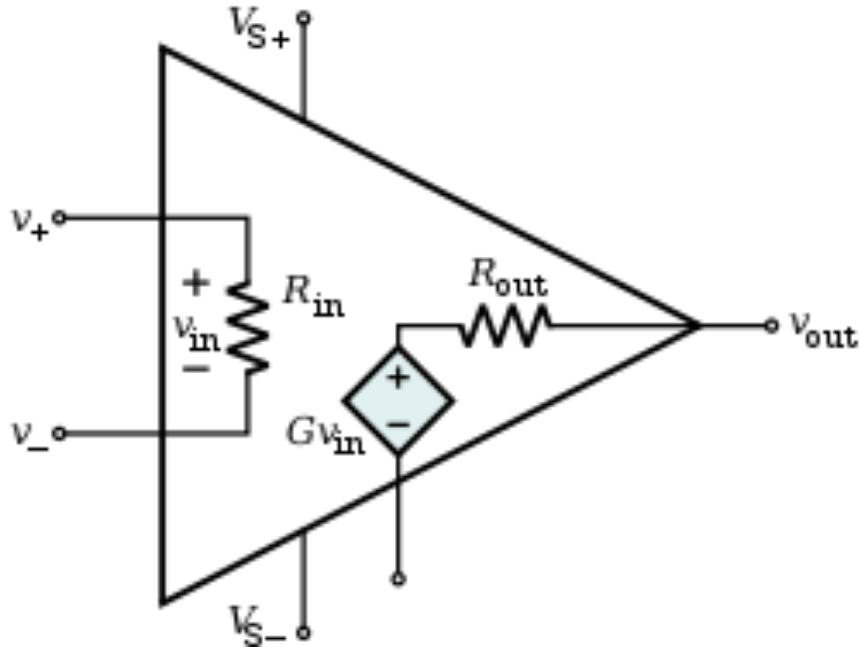
\includegraphics[width=0.3\textwidth]{images/opamp_model.png}
        } \\[5pt]
        \textit{Ideal} op-amps: $V_{out}$ is \textbf{INDEPENDENT of the load}. The \textit{internal voltage source} guarantees that $V_{out}$ is \textbf{kept the same}. & \\
        (\textit{But the current produced from the output can be different}.)
    \end{tabular}
\end{frame}